\chapter*{Preface}
\addcontentsline{toc}{fmbm}{Preface}
\addtocontents{toc}{\protect\enlargethispage{1\baselineskip}}


\section*{About this Book}

This book  covers foundational topics within computer vision, with an image processing and machine learning perspective. We want to build the reader's intuition and so we include many visualizations. The audience is undergraduate and graduate students who are entering the field, but we hope experienced practitioners will find the book valuable as well.

% This book does not pretend to review all existing works or provide exhaustive coverage of the field. There are other sources where the reader can get that information. Instead, here we cover some selected foundational topics within computer vision, with an image processing and machine learning perspective, and cover those formulations in detail. Our goal is to give you the material needed to learn and for this reason we include many visualizations. The audience is undergraduate and graduate students that are new to the field.  

%In order to write this book, we have adopted the following guideline: if you set up a goal and you fail at it, then just set up another goal. The best way of reaching the finish line is by bringing the finish line to where we are standing. And this is what we did. 

Our initial goal was to write a large book that provided a good coverage of the field. Unfortunately, the field of computer vision is just too large for that.  So, we decided to write a small book instead, limiting each chapter to no more than five pages. Such a goal forced us to really focus on the important concepts necessary to understand each topic. Writing a short book was perfect because we did not have time to write a long book and you did not have time to read it. Unfortunately, we have failed at that goal, too. %Instead of being very long or short, this book which covers a selected set of topics in depth.

% 
\section*{Writing this Book}

To appreciate the path we took to write this book, let's look at some data first. \Fig{\ref{fig:evolution_pages}} shows the number of pages written as a function of time since we mentioned the idea to MIT press for the first time on November 24,  2010.


\begin{figure}
    \centerline{
        \includegraphics[width=1\linewidth]{figures/preface/book_evolution_final.eps}
    }
    \caption{Evolution of the number of pages written as a function of time.
    }
    \label{fig:evolution_pages}
\end{figure}


Writing this book has not been a linear process. As the plot shows, the evolution of the manuscript length is non-monotonic, with a period when the book shrank before growing again. Lots of things have happened since we started thinking about this book in November 2010; yes, it has taken us more than 10 years to write this book. If we knew on the first day all the work that is involved in writing a book like this one there is no way we would have started. However, from today's vantage point, with most of the work behind us, we feel happy we started this journey. We learned a lot by writing and working out the many examples we show in this book, and we hope you will too by reading and reproducing the examples yourself.

When we started writing the book, the field was moving ahead steadily, but unaware of the revolution that was about to unfold in less than 2 years. Fortunately, the deep learning revolution in 2012 made the foundations of the field more solid, providing tools to build working implementations of many of the original ideas that were introduced in the field since it began. During the first years after 2012, some of the early ideas were forgotten due to the popularity of the new approaches, but over time many of them returned. We find it interesting to look at the process of writing this book with the perspective of the changes that were happening in the field. \Fig{\ref{fig:evolution_pages}} shows some important events in the field of artificial intelligence (AI) that took place while writing this book.


\marginnote{Starting to write this book was like entering this cave.
    \\[6pt]
    \centerline{
        \includegraphics[width=.4\linewidth]{figures/preface/cave.jpg}
    }
    \\[6pt]
    We had no idea what we were getting into.
}

\section*{Structure of the Book}

Computer vision has undergone a revolution over the last decade. It may seem like the methods we use now bear little relationship to the methods of 10 years ago. But that's not the case. The names have changed, yes, and some ideas are genuinely new, but the methods of today in fact have deep roots in the history of computer vision and AI. Throughout this book we will emphasize the unifying themes behind the concepts we present. Some chapters revisit concepts presented earlier from different perspectives.

One of the central metaphors of vision is that of multiple {\bf views}. There is a true physical scene out there and we view it from different angles, with different sensors, and at different times. Through the collection of views we come to understand the underlying reality. This book also presents a collection of views, and our goal will be to identify the underlying foundations.

The book is organized in multiple parts, of a few chapters each, devoted to a coherent topic within computer vision. It is preferable to read them in that order as most of the chapters assume familiarity with the topics covered before them. The parts are as follows:

{\bf Part I} discusses some motivational topics to introduce the problem of vision and to place it in its societal context. We will introduce a simple vision system that will let us present concepts that will be useful throughout the book, and to refresh some of the basic mathematical tools.

    {\bf Part II} covers the image formation  process.

    {\bf Part III} covers the foundations of learning using vision examples to introduce concepts of broad applicability.

    {\bf Part IV} provides an introduction to signal and image processing, which is foundational to computer vision.

    {\bf Part V} describes a collection of useful linear filters (Gaussian kernels, binomial filters, image derivatives, Laplacian filter, and temporal filters) and some of their applications.

    {\bf Part VI} describes multiscale image representations.

    {\bf Part VII} describes neural networks for vision, including convolutional neural networks, recurrent neural networks, and transformers. Those chapters will focus on the main principles without going into describing specific architectures.

    {\bf Part VIII} introduces statistical models of images and graphical models.

    {\bf Part IX} focuses on two powerful modeling approaches in the age of neural nets: generative modeling and representation learning. Generative image models
%, described in Part VII, 
are \textit{statistical image models} that create synthetic images that follow the rules of natural image formation and proper geometry. Representation learning seeks to find useful abstract representations of images, such as vector embeddings.

    {\bf Part X} is composed of brief chapters that discuss some of the challenges that arise from building learning-based vision systems.

    {\bf Part XI} introduces geometry tools and their use in computer vision to reconstruct the 3D world structure from 2D images.

    {\bf Part XII} focuses on processing sequences and how to measure motion.

    {\bf Part XIII} deals with scene understanding and object detection.

    {\bf Part XIV} is a collection of chapters with advice for junior researchers on effective methods of giving presentations, writing papers, and the mentality of an effective researcher.

    {\bf Part XV} returns to the simple visual system and applies some of the techniques presented in the book to solve the toy problem introduced in Part I.


%You will encounter convolutional neural networks (CNNs) in Chapter XX. CNNs are \textit{learnable} (Chapter XX) \textit{multiscale image pyramids} (Chapter XX) that use \textit{convolutional filters} (Chapter XX) as their basic operation. You will learn about generative adversarial networks (GANs) in Chapter XX. GANs are \textit{statistical image models} (Chapter XX) that create synthetic images that follow the rules of natural image formation (Chapter XX) and proper geometry (Chapter XX).

\section*{What Do We Not Cover?}

This should be a long section, but we will keep it short. We do not provide a review on the current state of the art of computer vision; we focus instead on the foundational concepts. We do not cover in depth the many applications of computer vision such as shape analysis, object tracking, person pose analysis, or face recognition.
%, 3D structure from motion and bundle adjustment, or vision and language. 
Many of those topics are better studied by reading the latest publications from computer vision conferences and specialized monographs.

\section*{Related Books}

We want to mention a number of related books that we've had the
pleasure to learn from.  For a number of years, we taught our computer vision class from the \textit{Computer Vision: A Modern Approach} by Forsyth and Ponce \cite{Forsyth2012}, and have
also used Rick Szeliski's book, \textit{Computer Vision: Algorithms and Applications} \cite{Szeliski2011}.  These are excellent general
texts.  \textit{Robot Vision}, by Horn  \cite{Horn86} is an older textbook, but covers
physics-based fundamentals very well.
The book that enticed one of us into computer
vision is still in print:  \textit{Vision}, by David Marr  \cite{Marr2010}.  The intuitions
are timeless and the writing is wonderful.

The geometry of vision through multiple cameras is covered thoroughly
in Hartley and Zisserman's classic, \textit{Multiple View Geometry in Computer Vision} \cite{Hartley2004}.  \textit{Solid Shape} \cite{KoenderinkSolidShape1990}, by
Koenderink, offers a general treatment of three-dimensional (3D) geometry.
Useful and related books include \textit{Three-Dimensional Computer Vision}, by
Faugeras \cite{Faugeras93}, and \textit{Introductory Techniques for 3D Computer Vision} \cite{Trucco1998},
by Trucco and Verri.

A number of recent textbooks focus on learning.  Our favorites are by
Mackay \cite{mackay2003information}, Bishop \cite{Bishop2006}, Murphy \cite{murphy2022}, and Goodfellow,
Bengio, and Courville \cite{Goodfellow-et-al-2016}.  Probabilistic models for vision are
well covered in the textbook of Simon Prince \cite{princeCVMLI2012}.

\textit{Vision Science: Photons to Phenomenology}, by Steve
Palmer \cite{Palmer1999}, is a wonderful book covering
human visual perception. It includes some chapters discussing
connections between studies in visual cognition and computer
vision. This is an indispensable
book if you are interested in the science of vision.

\textit{Signal Processing for Computer Vision}, by Granlund and Knuttson \cite{Granlund95},
covers many basics of low-level vision.  Ullman insightfully addresses
\textit{High-level Vision} in his book of that title, \cite{Ullman2000}.

Finally, a favorite book of ours, about light and vision, is
\textit{Light and Color in the Outdoors}, by Minnaert \cite{Minnaert2012}, a delightful treatment
of optical effects in nature.

\section*{Acknowledgments}

We thank our teachers, students, and colleagues all over the world who have taught us so much and have brought us so much joy in conversations about research. This book also builds on many computer vision courses taught around the world that helped us decide which topics should be included. We thank everyone that made their slides and syllabus available. A lot of the material in this book has been created while preparing the MIT course, ``Advances in Computer Vision.''

We thank our colleagues who gave us comments on the book: Ted Adelson, David Brainard, Fredo Durand, David Fouhey, Agata Lapedriza, Pietro Perona, Olga Russakovsky, Rick Szeliski, Greg Wornell, Jose María Llauradó, and Alyosha Efros. A special thanks goes to David Fouhey and Rick Szeliski for all the help and advice they provided. We  also thank Rob Fergus and Yusuf Aytar for early contributions to this manuscript. Many colleagues and students have helped proof reading the book and with some of the experiments. Special thanks to Manel Baradad, Sarah Schwettmann, Krishna Murthy Jatavallabhula, Wei-Chiu Ma, Kabir Swain, Adrian Rodriguez Muñoz, Tongzhou Wang, Jacob Huh, Yen-Chen Lin, Pratyusha Sharma, Joanna Materzynska, and Shuang Li.
Thanks to Manel Baradad for his help on the experiments in \chap{\ref{chap:simple_system_revisited}},  to Krishna Murthy Jatavallabhula for helping with the code for \chap{\ref{chapter:3D_multiview}},
and Aina Torralba for help designing the book cover and several figures.
%Special thanks to Alex Fito (\url{https://www.alexfito.es/}), a Mexican and Spanish illustrator, for designing our three cartoons in page 3, 

Antonio Torralba thanks Juan, Idoia, Ade, Sergio, Aina, Alberto, and Agata for all their support over many years.

%Antonio Torralba thanks Juan, Idoia, Ade, Sergio, Aina, Alberto, Pili, Sandra, Adrian, Agata, Pepe, Alex, Cristina, Carmen, Mariceli, and Tatito, for all their support over many years.

Phillip Isola thanks Pam, John, Justine, Anna, DeDe, and Daryl for being a wonderful source of support along this journey.

William Freeman thanks Franny, Roz, Taylor, Maddie, Michael, and Joseph for their love and support.

